
% !TEX encoding = Shift_JIS
% !TEX spellcheck = none



% 2019.01.04 初版
% 2020.05.11 改訂
%
% thesis.tex
%
%
%
%
\documentclass[10pt,twocolumn]{jsarticle}
\usepackage[dvipdfmx]{graphicx}	% 自分で加えた	by 野田
\usepackage{amsmath}			% 自分で加えた	by 野田
\usepackage{url}					% 自分で加えた	by 野田
\usepackage{comment}			% 自分で加えた	by 野田
\usepackage{supertabular}		% 自分で加えた	by 野田
\usepackage{cite}					% 自分で加えた	by 野田
\usepackage{here}				% 自分で加えた	by 野田
\usepackage[top=5truemm,bottom=15truemm,left=20truemm,right=16truemm]{geometry}

%●nag Detecting and warn?ing about obsolete LaTeX commands
%  http://www.ctan.org/tex-archive/macros/latex/contrib/nag
%  LaTeX文書の冒頭に
%\RequirePackage[l2tabu, orthodox]{nag}
%  と書いておくと古いコマンドやパッケージの利用を警告してくれます.
%
%●onlyamsmath  Inhibit use of non-amsmath mathe?matics markup when using amsmath
%  http://www.ctan.org/tex-archive/macros/latex/contrib/onlyamsmath
%\usepackage[all, warning]{onlyamsmath}
% で amsmath が提供しない数式環境を使用した場合に警告してくれます.

%\usepackage{secdot}
%\sectiondot{subsection}
%
%\makeatletter
%\def\section{\@startsection{section}{1}{\z@}%
%{1.5\Cvs \@plus.5\Cdp \@minus.2\Cdp}%
%{.5\Cvs \@plus.3\Cdp}%
%{\reset@font\centering\large\bfseries}}
%\makeatother

\title{
\flushleft{\large \textsf{X20-222}\\}
\centering{製造業向けロボットを知能化するアルゴリズムの研究}}
\author{●● ●● \hspace{10mm} 指導教員 野田 哲男}
\date{}

%
\begin{document}
%
% 表紙 および アブストラクト
%
\pagestyle{empty}
\maketitle
\small

\section{はじめに}
本稿は,卒業論文概要の作成要領を説明するものである.卒業論文概要は,発表会当日に配布される.卒業論文の内容を端的にまとめたものとする.A4サイズ(縦)1ページで作成する. 

\section{先行研究}
本稿は,卒業研究概要作成にあたっての指示,注意点をまとめたものである.フォーマットや書式は,日本ロボット学会の論文投稿要項[1]や,ロボット工学科学生実験テキスト[2]を参考に作成した.

\section{課題とその解法}
\subsection{課題} 
概要の構成は,学生番号,卒業研究タイトル名,指導教員名,本文,参考文献とする. レイアウトやフォントは,本稿に準じるものとする.
\subsection{レイアウト}
余白は上25 [mm], 下30 [mm],左20 [mm], 右16 [mm] とする.本文は2段組とし,文字は9ポイントとする.各コラムは全角26字とする.行間は1行を基本とするが,必要に応じ調整してよい. 
\subsection{作成上の注意事項}
「〜です」「〜ます」調ではなく,「〜である」調で書く.本文の章立ては任意である.野田研奥義(課題Challenge,解法 Solution,成果 Outcome)をいたるところで守るべし.オリジナリティ,新規性,独創性,有用性を主張すること.科学的に仮説と検証を繰り返すこと.のどごしを重視すること.略語・専門用語には注釈をつける.
数式は本稿3.3,図表は本稿3.4に従って作成する. 
適切に引用すること.本稿3.7に従い参考文献に. 
原則,句読点は「,」「.」,英数字は半角とする.SI単位系を用いるが,特定の分野で慣用的に用いられている単位についてはこの限りではない. 
\subsection{数式について}
数式は,原則として行の中央に置く. 式番は数式の右側に半角数字でふり,( ) で囲む.本文中で式を指示する場合は,式(1), 式(1)(2)などとする. 
\subsection{図表について}
図には通し番号の図番(Fig. 1, Fig. 2,... または図1, 図2,...)とタイトル(キャプション)を図の下に入れる.縦・横軸の外側中央にそれぞれ軸のタイトル(ラベル)を書く.ラベルは各軸のデータの意味と単位を記述し,単位は括弧で囲むこと.
表には通し番号の表番(Table 1, Table 2,... または表1, 表2, ...)とタイトル(キャプション)を表の上に入れる.表の行と列のデータの意味と単位を記述し,単位は括弧で囲むこと.
図表は上か下に固める.図1あるいはFig. 1, 表1あるいはTable 1などと本文から必ず引用する.
写真は,図.被写体が人の場合,個人が特定できないように加工するか,本人の承諾をとり図のキャプションに.
\subsection{参考文献について}
参考にした著書や論文がある場合は番号をふり,書誌情報(著者名,書名,引用ページ,出版社,発行年など)を最後の章にまとめて記載する.本文中の該当箇所に 参考文献番号を[1],[1,2],[1-3] のように明記する.
リストの書き方の流儀は様々だが提出先の指定するフォーマットに合わせるのが良い.R科卒論のごとく書式指定がない場合は,例えば日本ロボット学会の論文投稿規則( 
\url{https://www.rsj.or.jp/data_rules/F-02.pdf} のP15)に合わせることにすれはよい.
 
図1.装丁のフォーマット

\section{結論}
得られた結論を,定量的に評価せよ.2倍になった,など. 

\section{おわりに}
作成した原稿の提出期限と提出方法については,指導教員の指示に従う. 

%↓コンパイルされない
\if0
\begin{thebibliography}{}
\bibitem
論文・一般記事投稿用スタイルファイル(日本ロボット学会): \url{http://www.rsj.or.jp/journal/stylefile}, 2019年1月12日閲覧

\bibitem
前田:“レポート作成技法講習”,2014年度ロボット工学科学生実験Iテキスト,pp.1 -pp.9, 2014
\end{thebibliography}

\section*{本研究に関する発表リスト}
\begin{enumerate}
\renewcommand{\labelenumi}{[\arabic{enumi}]}
\item
高本,野田:ゼロ駆動うんたらかんたら,研究会ROOB2018

\item
高本,野田:セロ駆動うんたら,第19回計測自動制御学会システムインテグレーション部門講演会,1D3-211,pp.113-115, 2018

\end{enumerate}

\begin{figure}[b]\centering 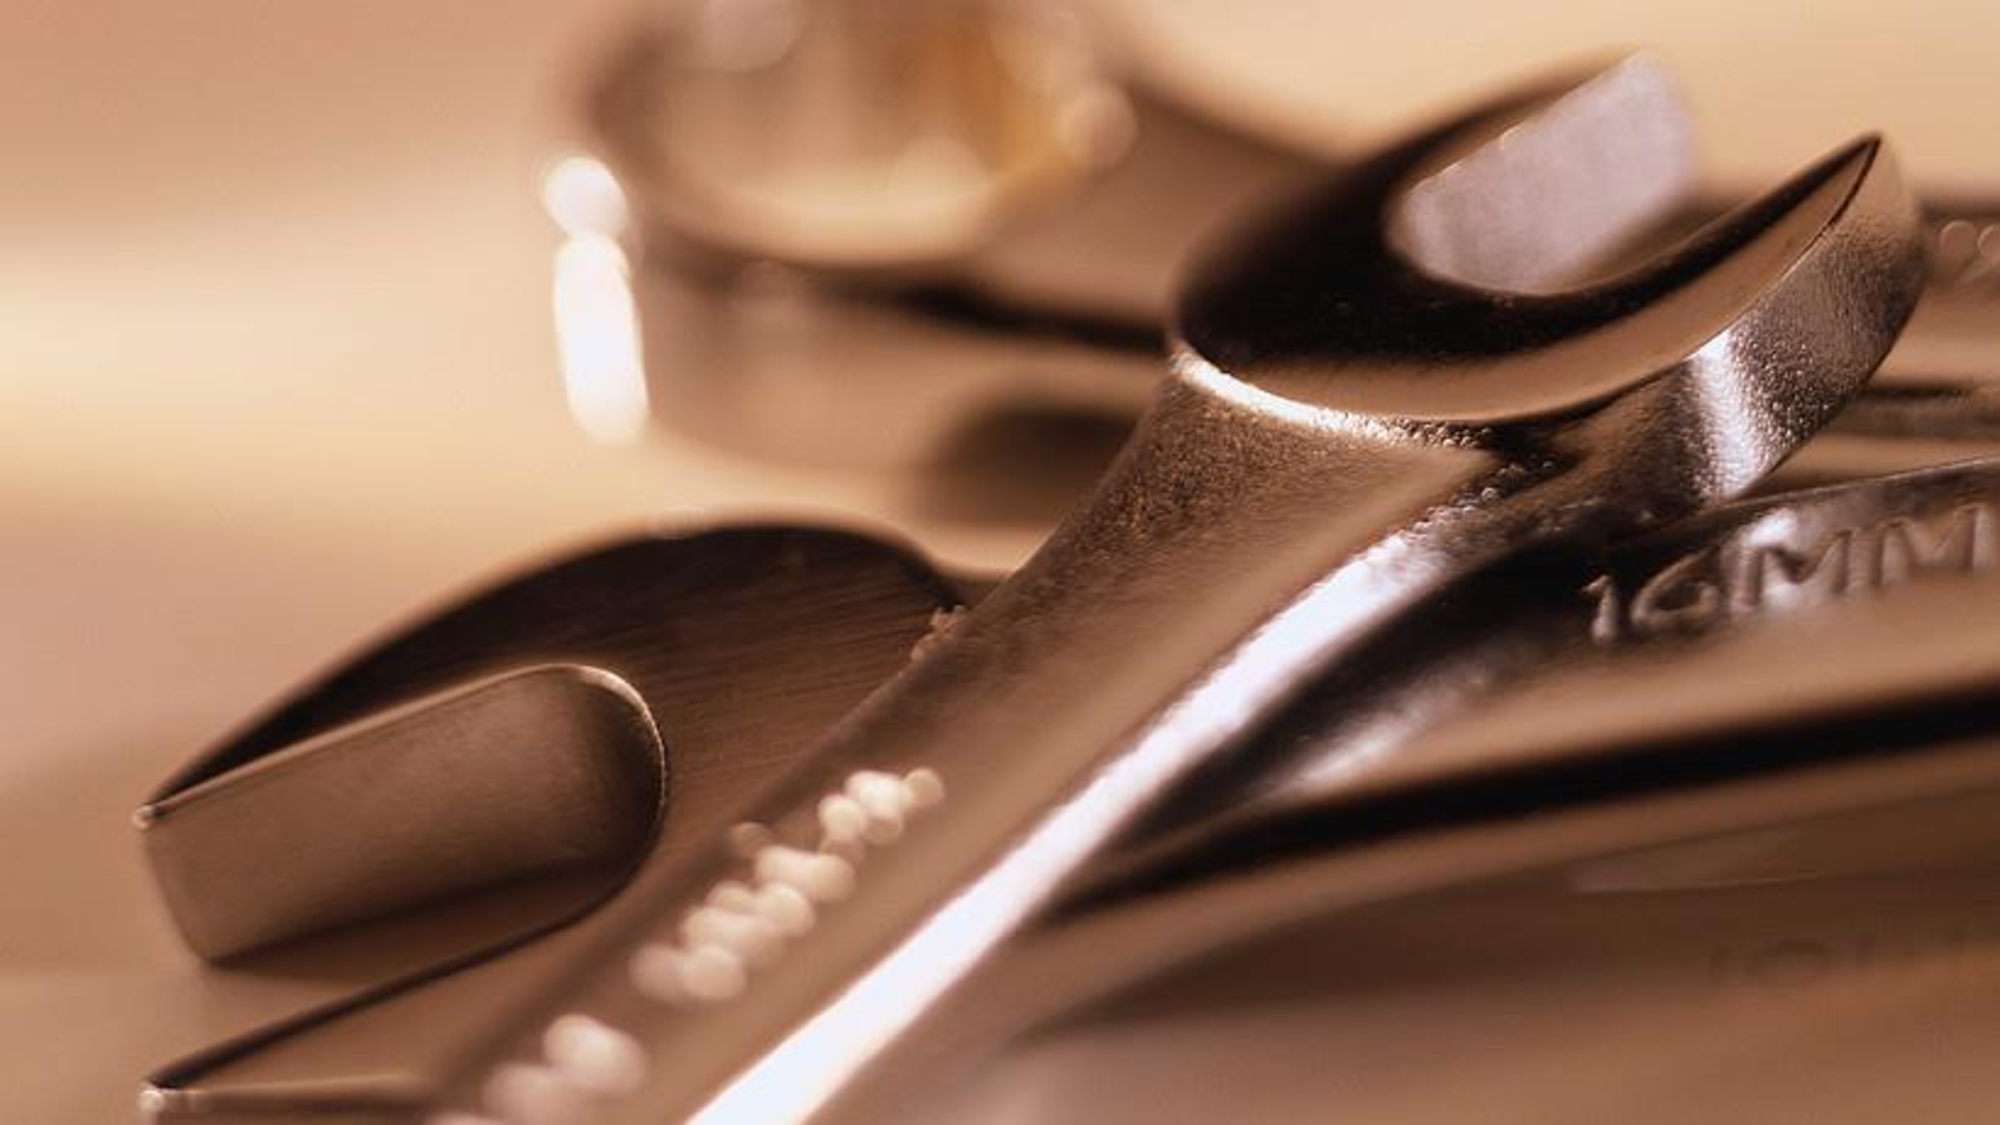
\includegraphics[width=5cm]{Fig/ChangesInManufacturing.pdf}
\caption{製造業におけるニーズとソリューション選択肢の変遷}\label{fig:ChangesInManufacturing}\end{figure}
\fi
%↑コンパイルされない

%参考文献
\small
\bibliographystyle{jrsj}
\bibliography{Reference}
\normalsize

\end{document}


